\chapter{Existing systems and technologies} 
\section{Existing systems}
This section discusses 4 existing visualisations that have a theme depicting
space or planets. Following the description, each visualisation is analysed to
discover which of the User Scenarios detailed previously existed within the
system.
\subsection{Worlds: The Kepler Planet Candidates - Non Interactive}
 This animation \cite{worlds} shows  planet candidates found by NASA's Kepler
mission. These candidates are animated in orbit around a single star. They are
drawn to scale with accurate radii, orbital periods, and orbital distances. They
range in size from 1/3 to 84 times the radius of Earth. Colors represent an
estimate of temperature with red indicating warmest, and blue indicating coldest
candidates. 
\begin{figure}[H]
  \centering
      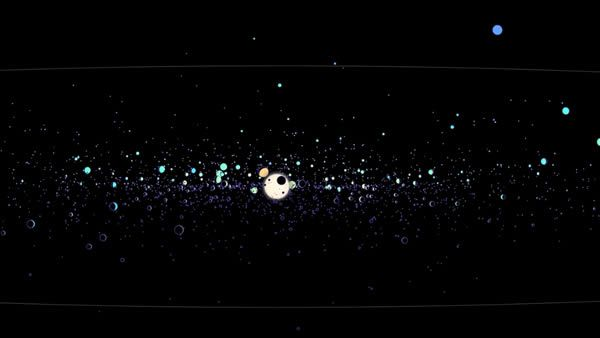
\includegraphics[width=0.8\textwidth]{images/worlds.jpg}
  \caption{Image of Worlds Visualisation}
\end{figure}
The layout of this animation is very similarly to the Kepler Visualisation Tool
that I am extending. This means that it provides insights into how my
visualisation can be improved as Worlds is a much more visually appealing
system. By researching how it displays its Exoplanets I can further improve my
own visualisation.
 \\\\
{\bf Scenario 1.} View planets ordered by their similarity to Earth:\\
Worlds has comprehensive functionality for comparing the different Exoplanets to
one another, however it does not offer any functionality regarding comparisons
to earth 
\\\\
{\bf Scenario 2.} Select ranges for attributes of each planet displayed:\\
Worlds does not offer any functionality for any filtering of Exoplanets, this
means that a user can only see all planets at once which can be overwhelming and
causes many of the exoplanets to be excluded from the user due to overlapping
and clustering. The reason that this is done is to convey how many Exoplanets
there are and how their scale differs among each Exoplanet
\\\\
{\bf Scenario 3.} Select planets to display more information:\\
Worlds is non interactive which means that users are not able to request further
information about the visualisation elements that they are seeing. This ability
to find out more is a key part of the interactive visualization that is needed
for this project.
\\\\
{\bf Scenario 4.} View planets in the same solar system:\\
Worlds shows all Exoplanets as if they are orbiting a single star. This allows
for each of them to be compared against one another easily. However this does
remove the ability for a user to see which planets are together in the same
solar system.


\subsection{The Kepler Orrery and The Kepler Orrery 2 - Non interactive}
The Kepler Orrery \cite{orrery} illustrates the exoplanet candidates in their
own solar systems. The orbit radii are to scale with respect to each other and
planet sizes are to scale with respect to each other, but orbits and planet
sizes are different scales. The colors are in order of semi-major axis:
two-planet systems (242 in all) have a yellow outer planet; 3-planet (85) green,
4-planet (25) light blue, 5-planet (8) dark blue, 6-planet (1, Kepler-11)
purple. 
\begin{figure}[H]
  \centering
      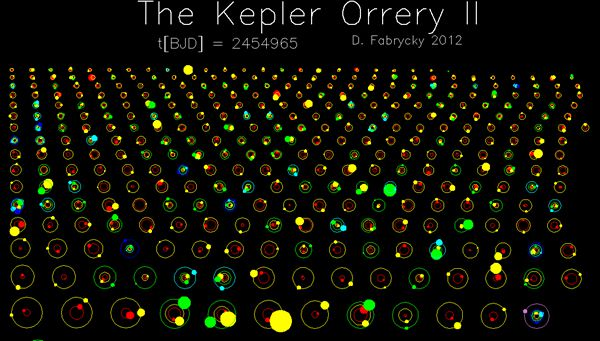
\includegraphics[width=0.8\textwidth]{images/orrery.jpg}
  \caption{Image of The Kepler Orrery Visualisation}
\end{figure}
This system exhibits small multiples, a grid of small similar graphics or
charts, allowing them to be easily compared. This provides insights into how I
can use small multiples to display information about groups of planets. This
will be important for displaying which planets share a solar system.
\\\\
{\bf Scenario 1.} View planets ordered by their similarity to Earth:\\
Like worlds, The Kepler Orrery shows the similarities between each of the
exoplanets but does not have the functionality to allow users to make a
comparison to earth and our own solar system.
\\\\
{\bf Scenario 2.} Select ranges for attributes of each planet displayed:\\
As The Kepler Orrery is non interactive it is not possible to change the ranges
of the Exoplanets being displayed. However due to the layout of the
visualisation, which uses small multiples by grouping each solar system into its
own visualisation element it removes a lot of the issue of overcrowding and
overlapping.
\\\\
{\bf Scenario 4.} View planets in the same solar system:\\
This visualisation uses small multiples to great effect at displaying the
groupings of each panel into each solar system. By displaying each planet
orbiting its own star it removes the risk of confusion about what the planet is
actually orbiting which could be the case with Worlds.

\subsection{Celestia - Interactive}
Celestia \cite{celestia} is a free real-time space simulation that lets you
visually experience the universe in three dimensions. It is an open source
system written in C++. 
\begin{figure}[H]
  \centering
      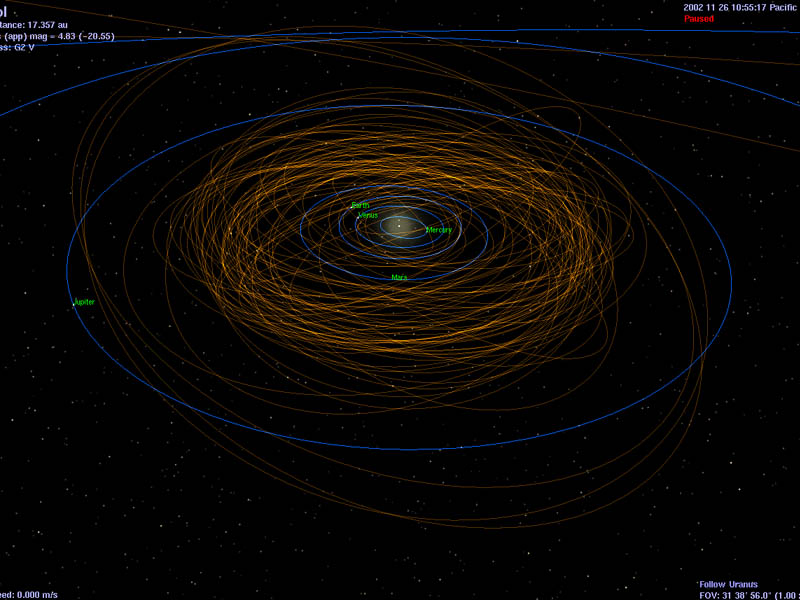
\includegraphics[width=0.5\textwidth]{images/celestia.jpg}
  \caption{Image of Celestia Visualisation}
\end{figure}
This visualisation is much larger and more encompassing system than is needed
for this project, as it is a full 3D space simulation. However is does offer
insights into how to effectively portray planets and their orbits (See Figure
2.3). It also provides textures that can be used in my visualisation to depict
what planets actually look like to increase user immersion.
\\\\
{\bf Scenario 1.} View planets ordered by their similarity to Earth:\\
Maybe
\\\\
{\bf Scenario 2.} Select ranges for attributes of each planet displayed:\\
Maybe
\\\\
{\bf Scenario 3.} Select planets to display more information:\\
Maybe
\\\\
{\bf Scenario 4.} View planets in the same solar system:\\
Maybe
\\\\
{\bf Scenario 5.} View the Goldilocks zones of each planet:\\
Maybe
\\\\
{\bf Scenario 6.} Select two planets to compare against one another:\\
Maybe\\\\
{\bf Scenario 7.} Navigate the visualisation with gestures: \\
Maybe\\\\
\subsection{Kepler Visualisation Tool}
An existing system built with Processing is the Kepler Visualisation
Tool\cite{kepler_github, kepler_article}. It is a simple visualisation focusing
on displaying the candidate Exoplanets temperatures and their locations in
relation to their distance from their nearest star, so that a sense of scale can
be perceived. Each candidate’s estimated size, orbital speed, and orbital
separation is accurately depicted, and each planet is color-coded according to
its estimated effective temperature.
\begin{figure}[H]
  \centering
      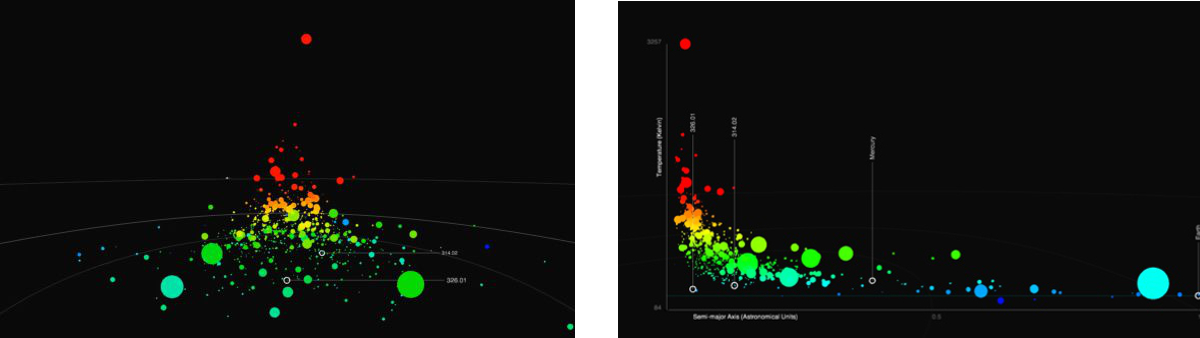
\includegraphics[width=1\textwidth]{images/kepler.jpg}
  \caption{Kepler Visualisation Tool Orbital View}
\end{figure}
% \begin{figure}[H]
%   \centering
%       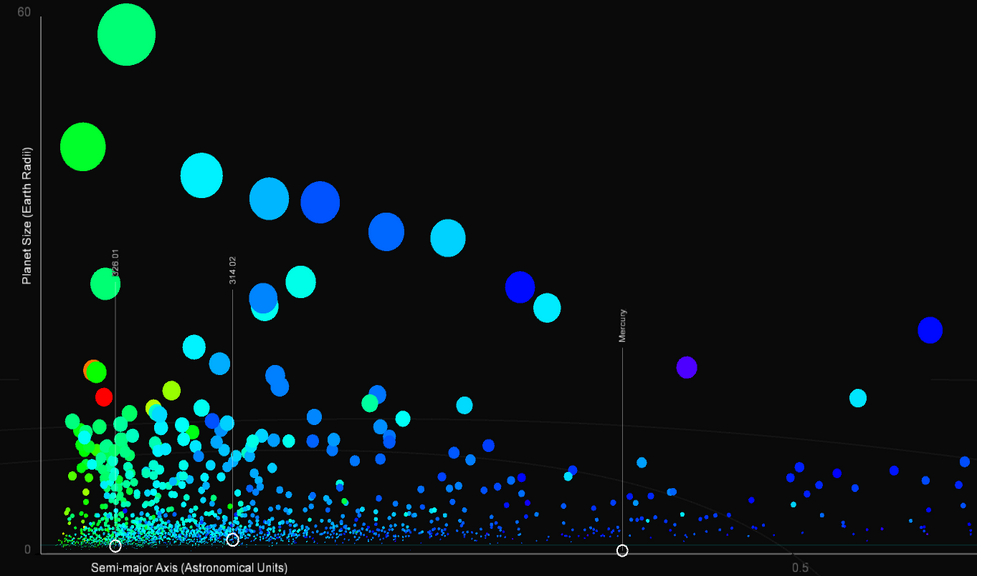
\includegraphics[width=0.8\textwidth]{images/kepler_graph.jpg}
%   \caption{Kepler Visualisation Tool Graph View}
% \end{figure}
The existing work in this system would serve as foundation for this project.
Because much of the visual aspects, and initial data manipulation of the
existing system are already complete. It means that implementing the features
needed for this projects completion could be focused on more heavily and larger
improvements to the existing system can be undertaken, such as better labeling
and information displays and user interaction methods.
\\\\
{\bf Scenario 1.} View planets ordered by their similarity to Earth:\\
Like Worlds and the Kepler Orrery, The Kepler Visualisation Tool has
functionality to display the similarity of each Exoplanet to each other.
However, it also has some limited functionality of comparing these to earth
which the others lack. It does this by displaying Earth, Mars, and Jupiter with
the same colours, size, and orbit speed as the Exoplanets. This gives a user a
chance to comprehend the scale and difference of some of the Exoplanets.
\\\\
{\bf Scenario 2.} Select ranges for attributes of each planet displayed:\\
The Kepler Visualisation Tool allows users to change which attributes the
planets are ordered by on the vertical plane (Y axis) ie, by size or
temperature, but does not allow users to select ranges of these attributes to
filter the Exoplanets

\subsection{Summary of Existing Applications}
\begin{figure}[H]
  \centering
      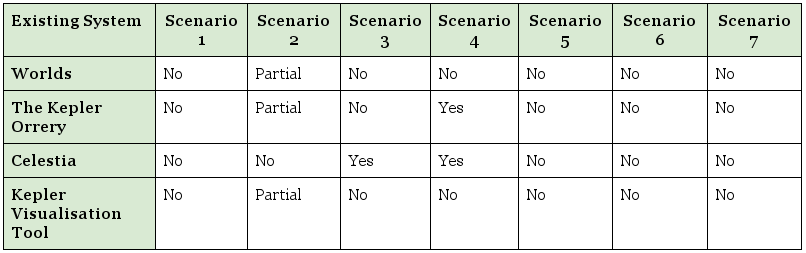
\includegraphics[width=1\textwidth]{images/existing.png}
  \caption{Matrix of existing solutions mapped to scenarios}  
    \label{fig:existing}
\end{figure}


\section{Analysis of technology options}
Many technologies were looked into and experimented with. Then the positives and
negatives of each option was weighed up before a decision was made about which would be the
suitable choice for the visualisation. It came down to 3 potential technologies that
would be suitable for the project, the next 3 subsections outline these in
detail.

\subsection{D3 (Data Driven Documents)}
D3 is a JavaScript library that allows the displaying of data in dynamic
graphics. Embedded
within an HTML web page, the JavaScript D3.js library uses pre-built JavaScript
functions to
select elements, create Scalable Vector Graphic (SVG)[17] objects, style them,
and add transitions,
dynamic effects and tooltips. Large datasets can be easily bound to SVG objects
using
simple D3 functions to generate rich charts and diagrams. D3 was created because
of the
need for a balance of expressiveness, efficiency, and accessibility that
previous visualization
toolkits did not allow [4].

D3 allows the binding of input data to arbitrary input elements. This means that
the exoplanet dataset can easily be bound to SVG elements for creating visualizations. D3
adopts the W3C Selectors API to identify document elements queried. This results in a
rich but concise selection method of elements in a visualisation. It allows debugging thanks to Google chrome and other modern browsers
development tools. A downside to D3 is that it does not allow 3D diagrams, although it does
allow pseudo 3D by using the painters algorithm and 3D textures.

\subsection{Prefuse}
Prefuse is a set of software tools for creating rich interactive data
visualizations [13]. The
Prefuse toolkit provides a visualization framework for Java. It supports a set
of features
for visualizing and interacting with data. It provides optimized data structures
for tables,
graphs, and trees. It can be used to build standalone applications, visual
components embedded
in larger applications, and web applets. Prefuse to greatly simplifies the
process
of representing and efficiently handling data, mapping data to visual
representations (e.g.,
through spatial position, size, shape, color, etc), and interacting with the
data.
To use Prefuse a basic familiarity with the Java is required, including setting
up and building
Java projects. A knowledge of Swing or another similar user interface toolkit is
also
useful for understanding some of the concepts behind Prefuse and for integrating
Prefuse
visualizations into larger applications. Experience with database systems is
also helpful. 
However the complexity of Prefuse means that the learning curve will be out of
scope for
this project.

\subsection{Processing}
Processing is an open source programming language and development environment
that was initially created to serve as a software
sketchbook and to teach the fundamentals of computer programming with a visual
context.
Using processing would mean that the visualization could be built with Java
while still using
a successful visualisation framework. The most complete existing visualization
using
the same exoplanet dataset (Kepler Visualization Tool) is built using
Processing.
Using this solution would involve learning the Processing language, however
Processing
is a library built in Java so the syntax is the same. This means the learning
curve should be shallow.
Using processing means that 3D elements could be included, this wouldn't be
possible with D3.

\subsection{Decision of technology}
The final decision of technology was to use Processing, this is because it had
many positive aspects that the others did not and minimal negatives as the below
table illustrates.
\clearpage
\begin{figure}[H]
  \centering
      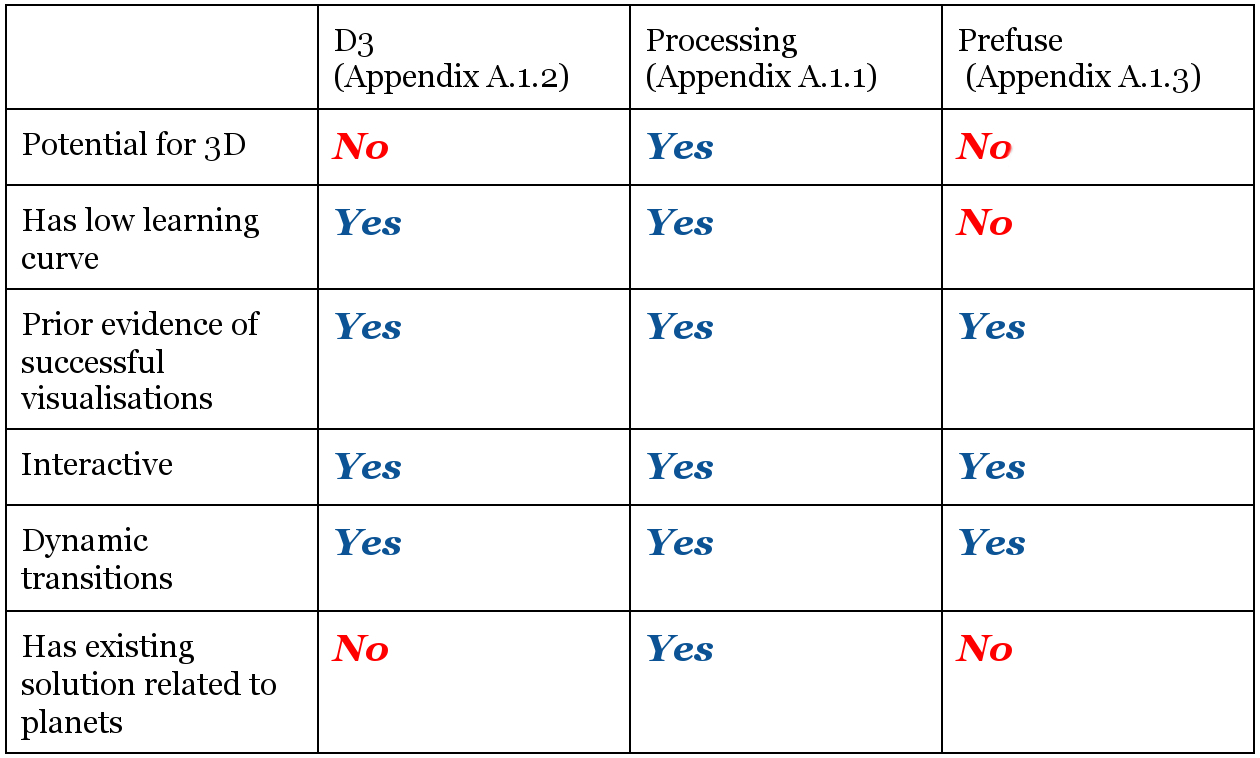
\includegraphics[width=0.8\textwidth]{images/table_technologies.jpg}
  \caption{Table of technology choices}
\end{figure}

As this project was created using Processing, it allowed me to extend the
previous visualisation using the same data set, The Kepler Visualisation Tool
\cite{kepler_github, kepler_article}. As the time was short for this project
building upon a previous solution increased the amount of progress that could be
made in the time afforded.

Taking this approach meant that the languages being used would be Java using
processing libraries. 

As this is such a large project involving many different iterations, version
control was important for maintaining records and backups of important changes
which was stored on remote servers to ensure against file loss in system
failures.
